\lab{Computing with Cython}{Cython}
\label{lab:Cython}
\objective{Use Cython to avoid the overhead of some parts of the Python language.}

Python is reasonably fast for computing the solutions to small problems.
However, for large computations Python quickly becomes unable to solve anything in a reasonable amount of time.
Why then is Python used if it's so slow?  One important answer to this question is programmer productivity.
The amount of time required to write code is dramatically less than the time required by low-level programming languages.

Low-level languages like C are renowned for their speed.
These languages are compiled to machine code that is better adapted on a computer's processor.
When a C program adds two numbers together, we have to be very specific about what two numbers are added together.
The computer can understand basic data types such as integers, floats, and arrays.
Python represents each of these data types using its own objects.
These are objects are generally fast and we don't notice much the incurred overhead.
Over large calculations, the computational cost of these objects is compounded and can slow things down tremendously.
In these cases, we need to be able to access the machine-level data types for integers, floats, and strings for maximum efficiency.
A common way of doing this is to write slower portions of the code in a lower-level, compiled language.
This is usually accomplished by writing a C-extension for Python.
A C-extension is a module that can be used like a Python module, but is written in C.
Python is written in C, and it has well-defined ways to perform operations on Python objects from C.
This enables performance critical code to be executed as fast as possible in a Python environment.
Writing these C-extensions can often be difficult and tedious work.

Much of the time, the operations that are performed in these C extensions are direct analogs of simple operations from either Python or C, but the interface for working with both languages simultaneously often complicates what would otherwise be a series of simple operations.
Cython was created to automate the creation of these C extension modules.
As a language, \textbf{it is essentially just Python with some extra type declarations.}
Using Cython, C-extensions can be written very quickly and give all the benefits of C speed.
Cython also makes it easier to avoid bugs (like memory leaks) that often arise when writing C extensions.

Cython is like Python with added syntax that enables you to call C functions and declare C types on Python variables.
The additional type declarations of Cython allow it to generate highly optimized C code that will compile with all major C/C++ compilers.
Beginning users often use it to speed up loops and array access times.
It is often used to create Python interfaces for C and C++ libraries and to write well-optimized Python libraries.
Since Cython outputs C code, you can easily call any C function from any point in your Python program.

Cython is used extensively in many packages.
SciPy uses Cython extensively in many of its packages for both improved speed and creating interfaces to packages that are written in C or C++.
It also uses a tool called f2py to interface with Fortran (another fast programming language).
Most core NumPy operations are written exclusively in C, but some of the components in its \li{random} module are written in Cython.
Several other packages like pyfftw, pandas, scikit-learn, scikit-image, and astropy use Cython extensively.
The package Kivy, that is used to write Android and iOS apps in Python, relies heavily on Cython.
The computer algebra system Sage also relies very heavily on Cython to write fast code and interface between the many different packages it uses.

\begin{warn}
Don't expect Cython to speed up Python code automatically.
If you run unmodified Python code through the Cython compiler, the result may be somewhat faster, but it may not.
The benefits from Cython come when you change some portions of your code (like loops and operations that are performed inside loops) so that they are performed in C and no longer need to use generic Python objects.
\end{warn}

\begin{warn}
Poorly written code will not perform well, regardless of the language in which it is written.
It is often easier and more effective to focus on writing good code in Python than it is to try to interface with a different ``faster" language.
If you need to speed up your code, first profile it to see which parts are slow (IPython's magic function \li{\%prun} can be used for this), then focus on removing unneeded operations from the slow portion of your code.
Effective use of array operations in NumPy can often make code simpler and faster than it would have been if you had tried to write all the operations yourself in C, Fortran, or any other language.
Cython should be used when other attempts at optimization and vectorization are insufficient or when you need to use functionality from a C or C++ library that is not available in Python.
\end{warn}

\section*{Compilation}

Cython has a more complex compilation process than Python and is not usually run interactively.
Cython code is usually written in a \texttt{.pyx} file.
Such a file is then compiled to C, and then the C is compiled to machine code.
The resulting file is a Python extension that can be imported from the Python interpreter.
Many of the same built in features, data types, and functions from Python work in Cython, but keep in mind that too many calls to Python based functions may slow down a Cython program.
Figure \ref{cython:compilation} shows how a Cython file is compiled and how a function call to a Cython module works.
Regardless of what method you use to compile a Cython file, this is more or less how it works.

\begin{figure}
\centering
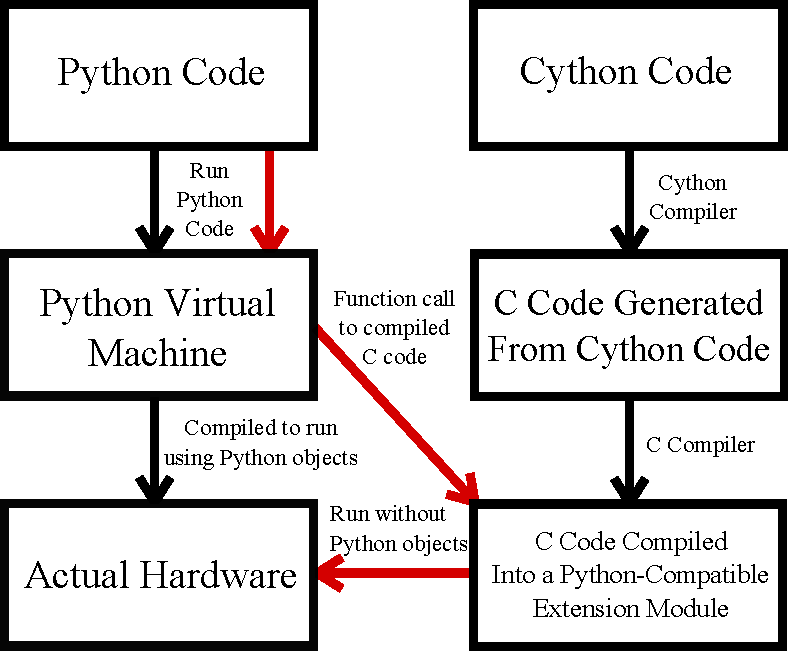
\includegraphics[width=\textwidth]{compilation.pdf}
\caption{A diagram of how Cython compilation and calls to Cython functions work.
The path from using a Cython function in a Python file to the actual evaluation is shown in red.}
\label{cython:compilation}
\end{figure}

There are a variety of ways to import Cython functions and classes into Python.
For example, consider the following cython file
\lstinputlisting[style=fromfile, language=Python]{hello.pyx}
We can compile this module using the following Python script:
\lstinputlisting[style=fromfile, language=Python]{setup.py}
This script should be used from the command prompt using the command:
\begin{lstlisting}[style=ShellInput]
python setup.py build_ext --inplace
\end{lstlisting}
After compiling the module, if the Python interpreter is running from the directory where the module was compiled, in Python the function can now be imported and run like any other Python function.
\begin{lstlisting}
from hello import hello
hello()
\end{lstlisting}
For larger projects and pieces of code that need special compilation options, using some sort of setup script is the best option.

This code can be compiled and imported in the IPython Notebook all in one step using the Cython magic function.
IPython must first import the corresponding functions so that you can use them.
With older versions of IPython and Cython you can import this magic function by running the command
\begin{lstlisting}
%load_ext cythonmagic
\end{lstlisting}
With newer versions of IPython and Cython, you should use the command
\begin{lstlisting}
%load_ext Cython
\end{lstlisting}
Once this magic function has been loaded, you compile the the \li{hello} function and import it by running the cell
\begin{lstlisting}
%%cython
def hello():
    print "Hello from Cython!"
\end{lstlisting}
The IPython magic function for Cython is good for compiling and experimenting with short snippets of code.

\begin{info}
When Cython generates the C file that is used to create the Python extension, it can show which portions of the code compile to Python operations and which portions compile to C operations.
This is called code annotation.
From the command line, if you were compiling \li{hello.pyx}, you could run the command
\begin{lstlisting}[style=ShellInput]
cython -a hello.pyx
\end{lstlisting}
This will generate a \li{html} file that you can open with your web browser.
It will show the lines that use Python in bright yellow and lines that use C in white.
Lines that use Python have a \li{+} to the left that expands the line of Cython code to show the relevant portion of C code that was generated.

The IPython Notebook magic can also show this information below a Cython-compiled cell.
This is done by replacing \li{\%\%cython} with \li{\%\%cython -a}.
\end{info}

\section*{Type Declarations}
One of the easiest ways improve performance in Cython is to declare types on variables.
Python does not enforce strict type checking.
Any variable can be any type and that type can change at any time.
To allow this behavior, an extra interface layer is needed.
Cython allows us to declare a variable of a certain type.
These typed variables are not Python objects, but native machine-types.

In Python, you can iterate over a list, or use a generator object.
In C, for-loops are managed by indexing an integer and checking to see if it is within a range of allowed values.
This is a good example of how using Python objects for everything can slow things down.
In Python a for-loop from 0 to 1000000 would look something like this:
\begin{lstlisting}
for i in range(1000000):
    pass
\end{lstlisting}
This for-loop creates a Python list of 1000000 objects and then iterates through it.
This can  be very slow.
It also uses a sizeable chunk of memory for no particular reason.
We can improve on this by using the \li{xrange} function as follows:
\begin{lstlisting}
for i in xrange(1000000):
    pass
\end{lstlisting}

Rather than making a list, \li{xrange} makes a generator object that returns the values as needed.
For large lists, this can give be a few times faster.
Cython will run this loop roughly the same way that Python would.
If, however, we pre-define the type of the loop variable, Cython will change the loop so that it is run in C.
A \li{cdef} statement can be used to define \li{i} as a C integer type with the syntax \li{cdef <type> <name>}.
The empty for-loops above may be written in Cython as follows:
\begin{lstlisting}
cdef int i
for i in range(1000000):
    pass
\end{lstlisting}
You can use a \li{cdef} statement to define multiple multiple variables of multiple types at once and initialize each of them to different values.
\begin{lstlisting}
# Declare integer variables i, j, and k.
# Set k equal to 2.
cdef int i, j, k=2

cdef:
    # Declare and initialize m equal to 4 and n equal to 5.
    int m=4, n=5
    # Declare and initialize e equal to 2.71.
    double e = 2.71
    # Declare a double precision complex number a.
    double complex a
\end{lstlisting}

Because Cython uses the extra type information, it can translate the loop into C, resulting in a speed-up of a factor of 50 over Python.
Cython achieves this speed-up by removing the cost of working with Python integer objects.
Similarly, when summing a large array of double precision floating point values, declaring the variable type will speed up the computation.
It is much easier for a computer to perform arithmetic operations without having to infer what datatypes are being used when each operation is performed.
Generally, whenever a large number of computations involve the same data type, adding type declarations should speed things up considerably.

Table \ref{table:cython_types} shows the different numeric types that are available in Cython.
Cython uses the same type naming conventions as C and C++.
On most normal modern systems, the sizes listed for integers will apply, though some are still dependent on the operating system.

\begin{table}
\begin{center}
\begin{tabular}{|p{2.8cm}|p{2.5cm}|p{6cm}|}
\hline
Cython Type & NumPy Type& Description \\
\hline
float & float32 & 32 bit floating point number \\
double & float64 & 64 bit floating point number \\
float complex & complex64 & 64 bit floating point complex number \\
double complex & complex128 & 128 bit floating point complex number \\
char & int8 & 8 bit signed integer \\
unsigned char & uint8 & 8 bit unsigned integer \\
short & int16 & 16 bit signed integer \\
unsigned short & uint16 & 16 bit unsigned integer \\
int & int32 & 32 bit signed integer \\
unsigned int & uint32 & 32 bit unsigned integer \\
long & int32 or int64 & 32 or 64 bit signed integer (size depends on platform) \\
unsigned long & uint32 or uint64 & 32 or 64 bit unsigned integer (size depends on platform ) \\
long long & int64 & 64 bit signed integer \\
unsigned long long & uint64 & 64 bit unsigned integer \\
\hline
\end{tabular}
\end{center}
\caption{Numeric types available in Cython.}
\label{table:cython_types}
\end{table}

\begin{warn}
Integer types in C are different from Python's integer type.
Python's integer type works with arbitrarily large integers.
C integers can overflow.
When you declare the type of a variable in Cython to be some sort of integer, it is declared as a C integer type and can overflow.
\end{warn} 

You can also declare types for arrays.
Declaring types for arrays allows some operations involving arrays to be performed \emph{much} faster.
The \li{__getitem__} method (equivalent to array access using \li{[ ]}) of NumPy arrays is written for Python and requires roughly the same cost as a Python function call.
There are several ways to avoid this extra cost.
Cython does include an interface for C arrays and pointers, but the interface is not terribly convenient, so we will not discuss it here.
Fortunately, Cython includes a C-level interface for Numpy-like array objects.
Cython's arrays are called typed memoryviews.

A typed memoryview can be declared like this:
\begin{lstlisting}
cdef double[:,:] X = ...
\end{lstlisting}
Declaring arrays in this manner allows us to access individual items in a NumPy array at roughly the same speed we could access items in a C array.
Unfortunately, this fast array access only works when accessing \textit{one item at a time} from the array.
As of this writing, Cython's memoryviews only support accessing and writing to their entries.
Any mathematical operations involving arrays must be performed by numpy or be run element-by-element in a loop that passes over the array.
Memoryviews do allow you to pass slices of arrays from one Cython-defined function to another without the cost of a Python operation.

\begin{info}
Although typed memoryviews cannot be used directly for arithmetic, they can be passed as arguments to most numpy functions.
Numpy includes functions for all common arithmetic operations, all of which allow the specification of an output array.
For example, the operation \li{c = a + b} can be performed on typed memoryviews using the expression \li{c = np.add(a, b)} and the operation \li{c[:] = a * b} can be performed as \li{np.multiply(a, b, out=c)}.
This does require the cost of calling a Python function, as well as all the checks that NumPy runs on all of the arguments passed to its functions, but, when working with large arrays, it can be worth it.
\end{info}

\section*{Compiler Directives}
There are several compiler directives which may be passed to the Cython compiler to speed up array access.
By default, Cython checks to see if the indices used in array accesses are within the bounds of the array.
Cython also allows negative indexing the same way Python does.
These features incur some performance loss and may be removed after a program has been carefully debugged.
Compiler directives in Cython can be included as comments or as function decorators.
Directives included in comments will apply to the whole file, while function decorators will only apply to the function or method immediately following the decorators.
The comments to turn off bounds checking and negative indices are
\begin{lstlisting}
# cython: boundscheck=False
# cython: wraparound=False
\end{lstlisting}
To use the function decorators, first import the \li{cython} module by including the line \li{cimport cython} in your import statements.
The decorators are
\begin{lstlisting}
cimport cython
@cython.boundscheck(False)
@cython.wraparound(False)
\end{lstlisting}
When using these compiler directives, make absolutely sure that your program is \emph{not} using negative indices or accessing any array out of bounds.
Doing so could access and possibly modify or access some portion of memory that has not been allocated as part of an array.
That can either crash Python or cause unexpected behavior in a program.
It is usually best to only include these directives after debugging a program thoroughly.

Cython has many other compiler directives.
One to be aware of is the \li{cdivision} option.
In Python, the \li{\%} operator returns a number with the sign of the second argument, while C keeps the sign of the first argument.
In Python, \li{-1\%5} returns \li{4}, while in C, this returns \li{-1}.
Cython, by default, will behave like Python.
Cython will also check for zero division and raise a \li{ZeroDivisionError} when necessary.
This feature does have some cost.
If needed, you can make the \li{\%} operator behave like it would in C and turn off the check for zero division by setting \li{cdivision} to \li{True}.

\section*{Functions in Cython}
Type declarations can also be used for function arguments.
You can declare the types of the inputs for the function to ensure that it receives the right arguments.
\begin{lstlisting}
def myfunction(double[:] X, int n, double h, items):
    ...
\end{lstlisting}
Notice that the type declarations were not included for all of the arguments.
The untyped arguments are expected to be Python objects with the corresponding methods.
Computations involving these untyped arguments will use Python instead of C.
Keyword arguments are allowed for both typed and untyped arguments.

Cython also allows you to make C functions that are only callable within the C extension you are currently building.
These functions are declared using the same syntax as in Python, except the keyword \li{def} is replaced with \li{cdef}.
These functions can be called within the module, but are not actually imported into the Python namespace of the Python module.

Cython functions may be declared using the \li{cpdef} statement.
These functions are accesible within Cython without the cost of a Python function call, but can still be called from Python.
The return type for functions declared using \li{cdef} and \li{cpdef} may also be specified, for example:
\begin{lstlisting}
cpdef int myfunction(double[:] X, int n, double h, items):
    ...
\end{lstlisting}

\section*{Some Examples}
To show how to use Cython, we will take the dot product of two one-dimensional arrays.
This can be done in Python as follows:
\begin{lstlisting}
def pydot(A, B):
    tot = 0.
    for i in xrange(A.shape[0]):
        tot += A[i] * b[i]
    return tot
\end{lstlisting}
A C-compiled equivalent can be made using the following Cython code
\begin{lstlisting}
%%cython
cimport cython

@cython.boundscheck(False)
@cython.wraparound(False)
def cydot(double[:] A, double[:] B):
    cdef double tot=0.
    cdef int i
    for i in xrange(A.shape[0]):
        tot += A[i] * B[i]
    return tot
\end{lstlisting}
This function may be timed by evaluating the following cell in the IPython Notebook.
\begin{lstlisting}
from numpy.random import rand
n = 10000000
A = rand(n)
B = rand(n)
%timeit cydot(A, B)
\end{lstlisting}

Figure \ref{cython:dot} compares the timings of this new dot-product function with other possible implementations.

\begin{figure}
\centering
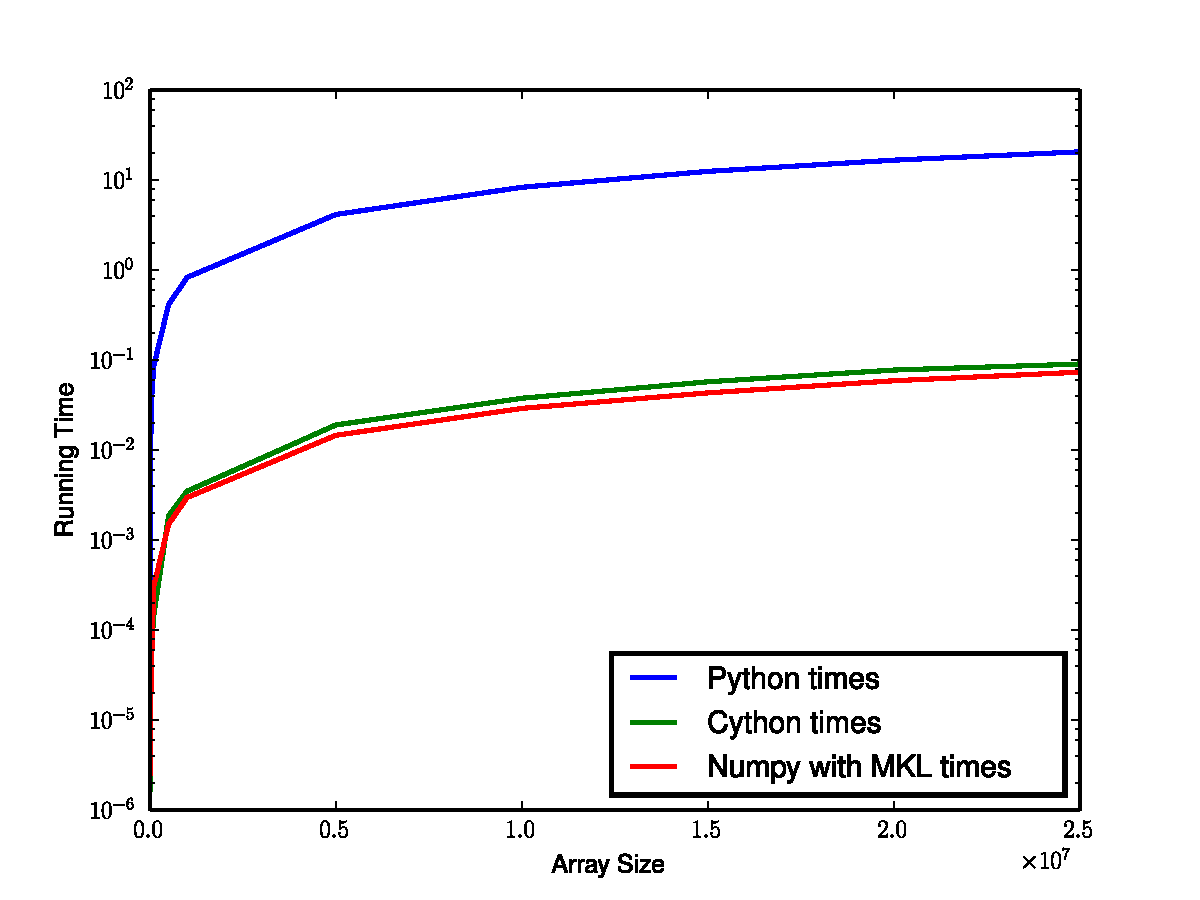
\includegraphics[width=\textwidth]{dot.pdf}
\caption{The running times of the pure Python dot-product, the Cython based dot-product, and the dot-product built into NumPy which links to the Intel MKL.
The Cython version can run nearly as fast as the version built into NumPy.}
\label{cython:dot}
\end{figure}

Now we will do a more advanced example using memoryviews.
We will write functions which, given a two-dimensional array \li{A}, make a new array \li{B} such that
\li{B[i,j] = dot(A[i],A[j])}.

Here's a purely iteration-based solution in Python:
\begin{lstlisting}
def pyrowdot(A):
    B = np.empty((A.shape[0], A.shape[0]))
    for i in xrange(A.shape[0]):
        for j in xrange(i):
            temp = pydot(A[i], A[j])
            B[i,j] = temp
        B[i,i] = pydot(A[i], A[i])
    for i in xrange(A.shape[0]):
        for j in xrange(i+1, A.shape[0]):
            B[i,j] = B[j,i]
    return B
\end{lstlisting}

To do this same sort of thing in Cython we can compile the following file:

\begin{lstlisting}
import numpy as np
cimport cython

@cython.boundscheck(False)
@cython.wraparound(False)
cdef double cydot(double[:] A, double[:] B):
    cdef double tot=0.
    cdef int i, n=A.shape[0]
    for i in xrange(n):
        tot += A[i] * B[i]
    return tot

@cython.boundscheck(False)
@cython.wraparound(False)
def cyrowdot(double[:,:] A):
    cdef double[:,:] B = np.empty((A.shape[0], A.shape[0]))
    cdef double temp
    cdef int i, j, n=A.shape[0]
    for i in xrange(n):
        for j in xrange(i):
            temp = cydot(A[i], A[j])
            B[i,j] = temp
        B[i,i] = cydot(A[i], A[i])
    for i in xrange(n):
        for j in xrange(i+1, n):
            B[i,j] = B[j,i]
    return np.array(B)
\end{lstlisting}

This can also be done in NumPy by running \li{A.dot(A.T)}.
The timings of the Python and Cython versions of this function are shown in Figure \ref{cython:rowdot}.

\begin{figure}
\centering
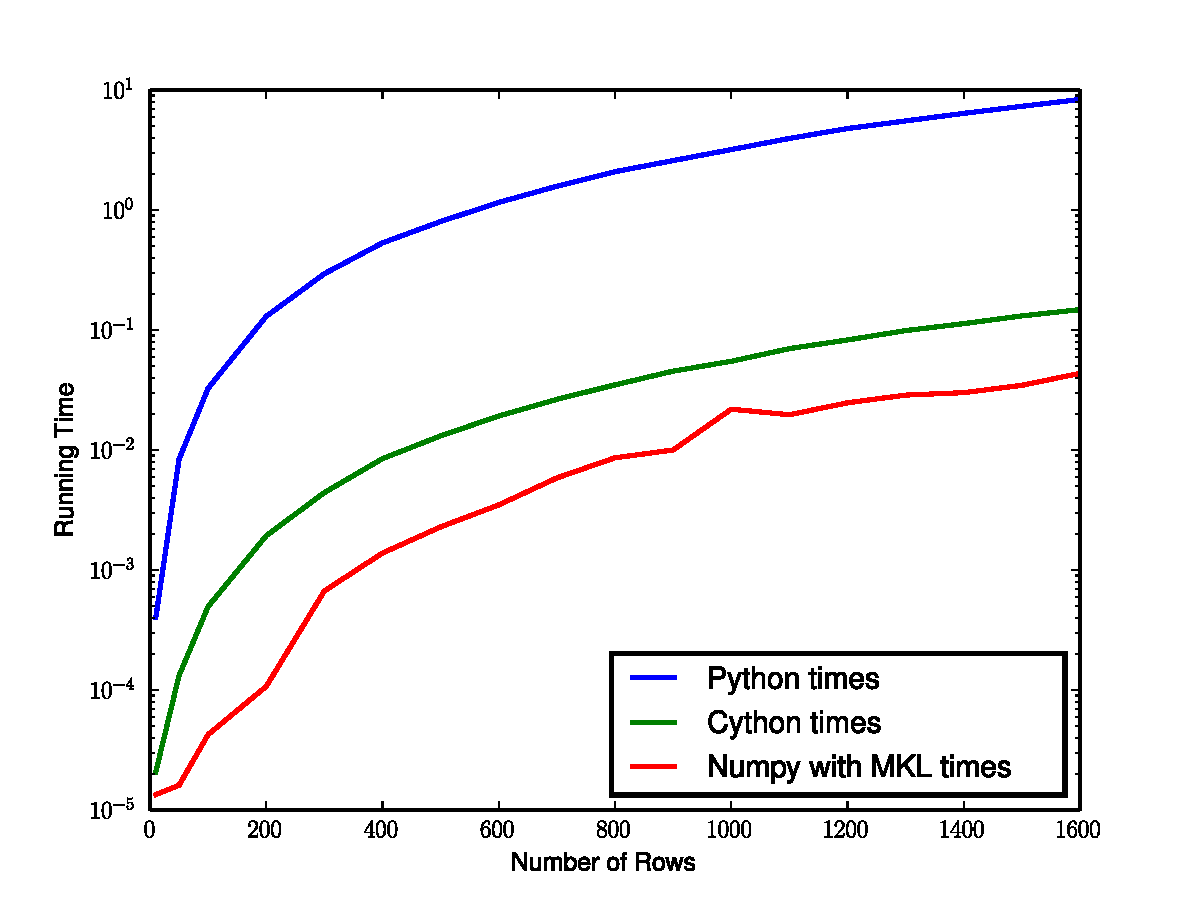
\includegraphics[width=\textwidth]{rowdot.pdf}
\caption{The times of the Python, Cython, and NumPy (with MKL) versions of the \li{rowdot} function that we used as an example.
The arrays used for testing were $n\times 3$ where $n$ is shown along the horizontal axis.}
\label{cython:rowdot}
\end{figure}

\begin{problem}
Write a function in Python that takes the sum of a one-dimensional array by iterating over it.

Write three Cython versions: one using a typed for-loop to iterate over the array, another using a typed for-loop and optimized array access, and another using a typed for-loop, optimized array access, and special compiler directives to further speed up array access.

Compare the speed of the functions you just wrote, the builtin \li{sum()} function and NumPy's \li{sum()} function.
What do you see?
Notice that when you specify the types for your variables in ways that don't work well, you may actually slow things down.
\end{problem}

\begin{problem}
In an earlier lab, you wrote a function to compute the LU decomposition of a matrix.
Write one version in pure Python that performs every operation element-by-element instead of using any sort of vector operation.
Port your new loop-based version to Cython.
Use typed for-loops, typed memoryviews, and the additional compiler directives in your optimized solution.
You may assume, in this case, that you are only dealing with real, two-dimensional arrays of double precision floating point numbers and that, as the computation proceeds, the diagonal elements will always be nonzero.
Compare the speed of your new solutions to the speed of the vectorized Python version you wrote earlier.
\end{problem}

\begin{problem} (optional)
The code below defines a Python function which takes a matrix to the $n$th power.
Port it to Cython.
Use typed for-loops, typed arrays, and the special compiler directives.
\begin{lstlisting}
import numpy as np
def pymatpow(X, power):
    prod = X.copy()
    temparr = np.empty_like(X[0])
    size = X.shape[0]
    for n in xrange(1, power):
        for i in xrange(X.shape[0]):
            for j in xrange(X.shape[1]):
                tot = 0.
                for k in xrange(size):
                    tot += prod[i,k] * X[k,j]
                temparr[j] = tot
            prod[i] = temparr
    return prod
\end{lstlisting}

Compare the speed of the Python function, the function you just wrote, and the \li{np.dot()} function.
The NumPy function should still be faster, but your solution should be much faster than the pure Python version.
NumPy and SciPy do this computation and other computations by calling BLAS and LAPACK.
BLAS and LAPACK are heavily optimized libraries for linear algebra.
The BLAS are usually implemented using a mix of C and assembly, while LAPACK is written exclusively in Fortran.
This is probably one of the best-optimized portions of NumPy and Scipy.
The difference in performance should be particularly clear in this case because of the high order of complexity of the algorithm.
\end{problem}

It is important to recognize that the choice of algorithm and fast implementation can both drastically affect the speed of your code.
A simple example is the tridiagonal algorithm which is used to solve systems of the form:
\[\begin{bmatrix}
b_0 & c_0 & 0 & 0 & 0 & \cdots & \cdots & 0 \\
a_0 & b_1 & c_1 & 0 & 0 & \cdots & \cdots & 0 \\
0 & a_1 & b_2 & c_2 & 0 & \cdots & \cdots & 0 \\
0 & 0 & a_2 & b_3 & c_3 & \cdots & \cdots & 0 \\
\vdots & \vdots & \vdots & \vdots & \vdots & \ddots & \ddots & \vdots \\
\vdots & \vdots & \vdots & \vdots & \vdots & \ddots & \ddots & c_{n-1} \\
0 & 0 & 0 & 0 & 0 & \cdots & a_{n-1} & b_n
\end{bmatrix}
\begin{bmatrix}
d_0\\
d_1\\
d_2\\
d_3\\
\vdots\\
\vdots\\
d_n
\end{bmatrix}
=
\begin{bmatrix}
x_0\\
x_1\\
x_2\\
x_3\\
\vdots\\
\vdots\\
x_n
\end{bmatrix}\]
The following Python code solves this system.
(\li{x} and \li{c} are modified in place)
The final result is stored in \li{x}, and \li{c} is used to store temporary values.
\begin{lstlisting}
def pytridiag(a, b, c, x):
    # Note: overwrites c and x.
    n = x.size
    temp = 0.
    c[0] /= b[0]
    x[0] /= b[0]
    for i in xrange(n-2):
        temp = 1. / (b[i+1] - a[i] * c[i])
        c[i+1] *= temp
        x[i+1] = (x[i+1] - a[i] * x[i]) * temp
    x[n-1] = (x[n-1] - a[n-2] * x[n-2]) / (b[n-1] - a[n-2] * c[n-2])
    for i in xrange(n-2, -1, -1):
        x[i] = x[i] - c[i] * x[i+1]
\end{lstlisting}

\begin{problem}
Port the above code to Cython using typed for-loops, optimized array accesses and the special compiler directives.
Compare the speed of your new function with the pure Python version given above.
Now compare the speed of both of these functions with the \li{solve()} function in \li{scipy.linalg}.
For your first two functions a good starting point for computation will be to consider $1000000 \times 1000000$ sized systems and then adjust the size so you get good results on your particular machine.
When testing the SciPy algorithm, you will probably want to start with systems involving a $1000 \times 1000$ matrix and then go up from there.
Keep in mind that the SciPy function is heavily optimized, but that it uses a much more general algorithm.

What does this example tell you about the relationship between good implementation and proper choice of algorithm?
In this case, the LU decomposition method used by the SciPy function has complexity $O(n^3)$, while the tridiagonal algorithm is $O(n)$.
\end{problem}

\begin{info}
Cython has predefined interfaces for many functions and classes in the C standard library.
These functions can be imported using a \li{cimport} statement.
\begin{lstlisting}
from libc.math cimport fabs, sin, cos, ...
\end{lstlisting}
Notice that we imported \li{fabs}.
This is the absolute value function from C.
The 'f' in \li{fabs} is short for floating point, since this function operates on floating point numbers.
\li{min} and \li{max} are also renamed the same way.
\end{info}